\documentclass[11pt]{article}
\usepackage[utf8]{inputenc}
\usepackage[T1]{fontenc}
\usepackage[a4paper]{geometry}
\usepackage[english,francais]{babel}
\usepackage{stmaryrd,amsfonts,amssymb,latexsym,amscd,amsmath,fancyhdr,amsthm}
\usepackage{graphicx}
\usepackage[printonlyused]{acronym}
\usepackage{algorithm}
\usepackage{algorithmicx}
\usepackage{algpseudocode}
\usepackage{listings}
\usepackage[usenames,dvipsnames]{color}

\definecolor{listinggray}{gray}{0.9}
\definecolor{lbcolor}{rgb}{0.9,0.9,0.9}
\lstset{
backgroundcolor=\color{lbcolor},
    tabsize=4,    
%   rulecolor=,
    language=[GNU]C++,
        basicstyle=\scriptsize,
        aboveskip={1.5\baselineskip},
        columns=fixed,
        showstringspaces=false,
        extendedchars=false,
        breaklines=true,
        prebreak = \raisebox{0ex}[0ex][0ex]{\ensuremath{\hookleftarrow}},
        frame=single,
        numbers=left,
        showtabs=false,
        showspaces=false,
        showstringspaces=false,
        identifierstyle=\ttfamily,
        keywordstyle=\color[rgb]{0,0,1},
        commentstyle=\color[rgb]{0.026,0.112,0.095},
        stringstyle=\color[rgb]{0.627,0.126,0.941},
        numberstyle=\color[rgb]{0.205, 0.142, 0.73},
%        \lstdefinestyle{C++}{language=C++,style=numbers}’.
}
\lstset{
    backgroundcolor=\color{lbcolor},
    tabsize=4,
  language=C++,
  captionpos=b,
  tabsize=3,
  frame=lines,
  numbers=left,
  numberstyle=\tiny,
  numbersep=5pt,
  breaklines=true,
  showstringspaces=false,
  basicstyle=\footnotesize,
%  identifierstyle=\color{magenta},
  keywordstyle=\color[rgb]{0,0,1},
  commentstyle=\color{OliveGreen},
  stringstyle=\color{red}
  }


\theoremstyle{plain} % style plain
\newtheorem{thm}{Théorème}
\newtheorem{rmq}[thm]{Remarque}
\newtheorem{exmpl}[thm]{Exemple}
\newtheorem{example}[thm]{Exemple}
\theoremstyle{definition} % style definition
\newtheorem{defi}[thm]{Définition}


\title{Runtime: Moteur d'exécution}
\author{Airbus Group Innovations}

\begin{document}
\maketitle

\newcommand{\mc}[1]{\mathcal{#1}}
\newcommand{\mcH}{$\mc{H}$}
\newcommand{\hmat}{$\mc{H}$-Matrice}
\newcommand{\hmats}{$\mc{H}$-Matrices}
\newcommand{\hvec}{$\mc{H}$-Vecteur}
\newcommand{\hvecs}{$\mc{H}$-Vecteurs}
\newcommand{\rkmat}{$\mc{R}k$-Matrice}
\newcommand{\rkmats}{$\mc{R}k$-Matrices}

\floatname{algorithm}{Algorithme}


\begin{abstract}
  Ce document donne des détails sur les principes de base et les algorithmes implémentés dans \textsc{runtime}, un moteur d'exécution utilisé par la bibliothèque \texttt{hmat}.
\end{abstract}

\tableofcontents

\section*{Acronymes}
\label{sec:acronymes}
\begin{acronym}[ccNUMA]
  \acro{aca}[ACA]{\emph{Adaptative Cross Approximation}}
  \acro{bem}[BEM]{\emph{Boundary Element Method}}
  \acro{bsp}[BSP]{\emph{Bulk Synchronous Parallel}}
  \acro{cfie}[CFIE]{\emph{Combined Field Integral Equation}}
  \acro{crbm}[CRBM]{Chambre Réverbérantes à Brassage de Mode}
  \acro{dag}[DAG]{\emph{Directed Acyclic Graph}}
  \acro{efie}[EFIE]{\emph{Electric Field Integral Equation}}
  \acro{fdtd}[FDTD]{Différences Finies en Domaine Temporel}
  \acro{fifo}[FIFO]{\emph{First In, First Out}}
  \acro{fmm}[FMM]{\emph{Fast Multipole Method}}
  \acro{hca}[HCA]{\emph{Hybrid Cross Approximation}}
  \acro{lifo}[LIFO]{\emph{Last In, First Out}}
  \acro{lpt}[LPT]{\emph{Longest Process Time}}
  \acro{mfie}[MFIE]{\emph{Magnetic Field Integral Equation}}
  \acro{mpi}[MPI]{\emph{Message Passing Interface}}
  \acro{numa}[ccNUMA]{\emph{Cache Coherent Non Uniform Memory Access}}
  \acro{ram}[RAM]{\emph{Random Access Memory}}
  \acro{sea}[SEA]{\emph{Statistical Energy Analysis}}
  \acro{ser}[SER]{Section Efficace Radar}
  \acro{shm}[SHM]{\emph{Structural Health Monitoring}}
  \acro{smp}[SMP]{\emph{Symmetric Multi-Processing}}
  \acro{spmd}[SPMD]{\emph{Same Program, Multiple Data}}
  \acro{svd}[SVD]{\emph{Singular Values Decomposition}}
  \acro{utd}[UTD]{\emph{Uniform Theory of Diffraction}}
\end{acronym}


\section{Introduction}
\label{sec:introduction}
\textsc{runtime} est un moteur d'exécution basé sur le modèle de graphe de tâches énuméré, similaire à celui utilisé par Quark et StarPU.
Il présente les caractéristiques suivantes~:~
\begin{itemize}
\item Mémoire partagée~;
\item MPI~;
\item Support limité de l'OOC (\emph{Out-Of-Core})~;
\item Différents ordonnanceurs, gestion des priorités (similaires à l'ordonnanceur \texttt{prio} de StarPU).
\end{itemize}

L'objectif de ce document est de documenter le fonctionnement de cet ordonnanceur, afin de faciliter ses évolutions et sa maintenance.
Après une présentation du modèle utilisé (ETF), nous donnerons son implémentation simple en mémoire partagée, puis documenterons les extensions nécessaires pour la gestion de la mémoire distribuée, et le support limité de l'OOC.


\section{Graphe de tâches enuméré}
\label{sec:graphe-de-taches}

\paragraph{Tâches et données}
\label{sec:taches-et-donnees}
Un algorithme peut être décomposé en un ensemble fini ordonné de tâches $T := \{t_i \ | \ i = 1, \dots, N \}$, opérant sur un ensemble de données $D = \{ d_j \ | \ j = 1,\dots, M\}$.
À chaque tâche $t \in T$ est associé deux ensembles de données respectivement lues et écrites par cette tâche, $In(t) \subset D$ et $Out(t) \subset D$.

\begin{example}[Produit Matrice-Matrice]
  \label{ex:gemm}
  Considérons l'opération $\textsc{gemm}(C, \alpha, A, B, \beta)$ définie par~:~
  \begin{equation*}
    C \gets \alpha A B + \beta C
  \end{equation*}
  Ici, $D = \{A, B, C \}$, $t = \textsc{gemm}$, $In(t) = \{A, B, C\}$ et $Out(t) = \{C\}$.
  Par ailleurs, si $\beta = 0$, alors $In(t) = \{A, B\}$.
\end{example}

\paragraph{Cohérence séquentielle}
\label{sec:cons-sequ}
Le modèle de cohérence utilisé ici est celui de la cohérence séquentielle.
Ceci signifie que le résultat final de toute exécution valide de l'algorithme est le même que celui d'une exécution dans laquelle les tâches sont exécutées séquentiellement dans l'ordre d'énumération.

La cohérence séquentielle peut être respectée en déterminant les tâches dépendantes, et en ajoutant une contrainte de précédence entre ces opérations, dont le sens est donné par l'ordre d'énumération des tâches.
Ces contraintes sont déterminées à partir des données lues et écrites par les tâches.

Plus précisément, soit $d \in D$,
\begin{itemize}
\item Toute \textbf{lecture} de $d$ nécessite que les \textbf{écritures} précédentes soient terminées~;
\item Toute \textbf{écriture} de $d$ nécessite que les \textbf{lectures} et \textbf{écritures} précédentes soient terminées.
\end{itemize}

Une tâche $t$ est une lecture de $d$ si et seulement $d \in In(t)$ (idem pour les écritures).
Notons $t_i \to t_j$ la relation ``$t_i$ doit précéder $t_j$''.
Alors,

\begin{equation}
  \label{eq:aretes-graphe-taches}
  \begin{array}{ccl}
    t_i \to t_j & \Longleftrightarrow & \exists d \in D,\ (d \in Out(t_{j})) \wedge (d \in In(d_i)) \wedge (i < j) \\
    & & \text{ou} \\
    & & \exists d \in D,\ (d \in In(t_{j}) \cup Out(t_{j})) \wedge (d \in Out(d_i)) \wedge (i < j)
  \end{array}
\end{equation}

La première relation traduit la condition ``une lecture doit attendre les écritures précédentes'', la seconde la condition ``une écriture doit attendre les lectures et écritures précédentes''.

Quelques remarques:
\begin{itemize}
\item Une tâche ne peut pas dépendre d'une tâche future (condition $i < j$)~;
\item Si $i \to j$ et $j \to k$, alors $i \to k$ (transitivité).
\end{itemize}

On définit alors le graphe de tâches par~:
\begin{defi}[Graphe de tâches]
  Soit $T$ et $D$ des ensembles de tâches et données définis tels que précédemment.
  On définit un graphe de tâche $G = (V, E)$ dont l'ensemble des sommets $V$ est $T$, et les arêtes $E$ sont $\{(t_i, t_j) \in T\times T \ |\  t_i \to t_j \}$.
  C'est un \textbf{graphe acyclique dirigé} (DAG).
\end{defi}

La transitivité de la relation $\cdot \to \cdot$ permet de simplifier l'expression du graphe (réduire son nombre d'arêtes), en introduisant~:
\begin{itemize}
\item Le dernier écrivain $W(d, t_i) := \{\max \{t_j \ |\  t_j < t_i \wedge d \in Out(t_j) \}\}$
\item L'ensemble des derniers lecteurs $R(d, t_i) := \{t_j \| \ d\in In(t_j) \wedge W(d, i) < t_j < t_i \}$
\end{itemize}
Le dernier écrivain de $d$ à l'instant de l'énumération de $t_i$ est la dernière tâche ayant écrit dans $d$ avant la tâche $t_i$, et les derniers lecteurs sont les lecteurs depuis la dernière écriture.

On définit alors le graphe de tâche réduit par~:
\begin{defi}[Graphe de tâches réduit]
  Soit $T$ et $D$ des ensembles de tâches et données définis tels que précédemment.
  On définit un graphe de tâche réduit $G = (V, E)$ dont l'ensemble des sommets $V$ est $T$.
  L'ensemble des arêtes $E$ de $G$ est construit ainsi~:
  \begin{align*}
    \forall t_i \in T,&\\
    &\forall d \in In(t), E \gets E \cup W(d, t_i) \ \text{et}\\
    &\forall d \in Out(t), E \gets E \cup W(d, t_i) \cup R(d, t_i)
  \end{align*}
\end{defi}

Ce graphe réduit encode les mêmes contraintes de précédence que le graphe initial, nous ne considérons que celui-ci dans la suite.

\begin{figure}[!htpb]
  \centering
  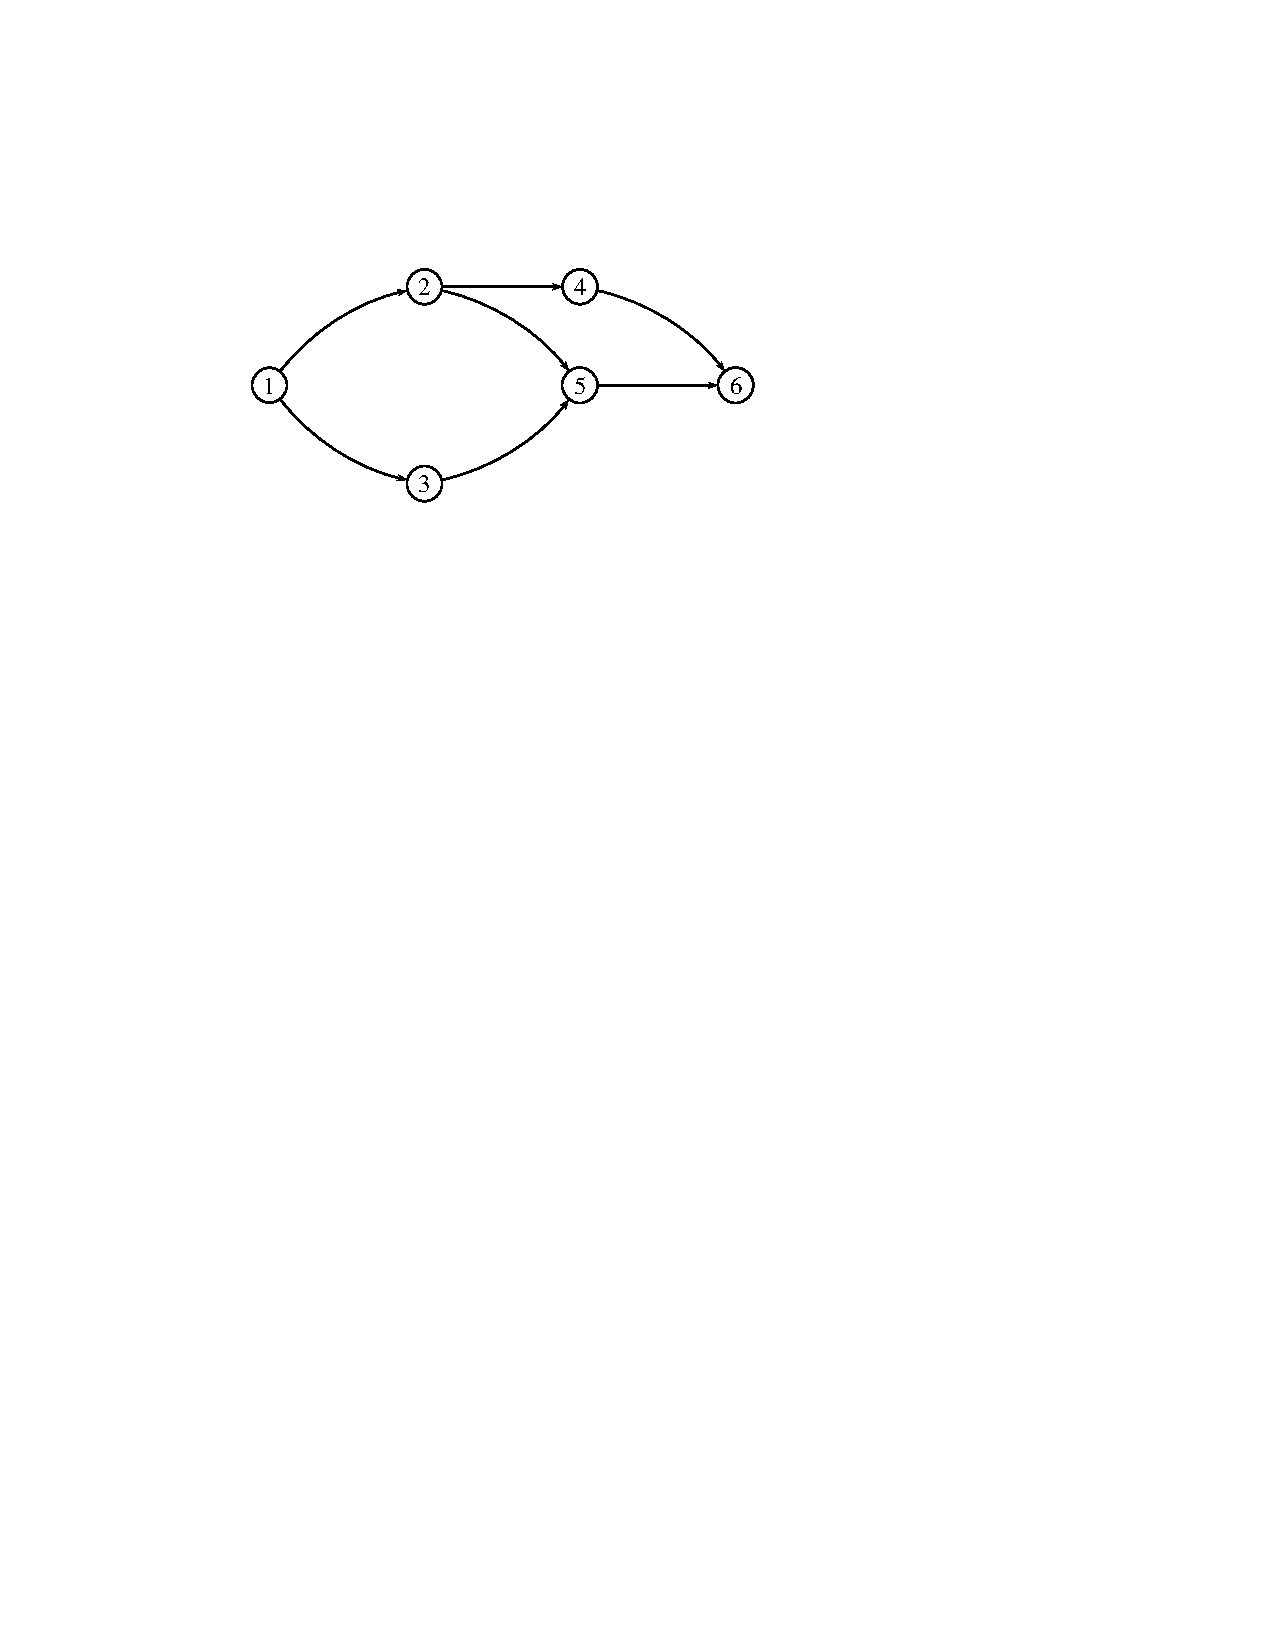
\includegraphics[width=8cm]{figures/dag_exemple.pdf}
  \caption{Exemple de graphe de tâches}
  \label{fig:exemple-dag}
\end{figure}

\section{Graphe de tâches et moteur d'exécution}
\label{sec:graphes-de-tache}

\paragraph{Exécution parallèle d'un graphe de tâches}
\label{sec:exec-parall-dun}
L'exécution parallèle des tâches du graphe de la figure~\ref{fig:exemple-dag} est claire~:~il est possible d'exécuter les tâches 2 et 3 en parallèle, mais il est également possible d'exécuter la tâche 4 en parallèle de la tâche 3, suivant les mêmes règles que celles définissant un parcours valide séquentiel.
Une tâche $t_i$ est considérée éligible pour exécution si toutes ses dépendances $\{t_{i'} \ |\ (i', i) \in A\}$ ont été exécutées.
Dans ce cas, l'exécution parallèle du graphe de tâches respecte la contrainte de cohérence séquentielle, et le résultat est le même quel que soit le nombre de processeurs.
Une propriété supplémentaire intéressante est même obtenue~:~les résultats sont dits exactement reproductibles.
Cette garantie n'est cependant plus valable dans le cas de l'utilisation d'extensions de ce formalisme, comme par exemple les réductions (qui ne sont pas supportées par \texttt{runtime}), les opérations de la norme IEEE-754 n'étant pas associative.


\subsection{Moteur d'exécution}
\label{sec:runtime}
Le formalisme de graphe de tâches exposé dans la section précédente a de nombreux avantages.
Il est expressif, simple, et la formalisation des contraintes permet une grande liberté d'exécution parallèle.
En effet, certaines méthodes de parallélisation sont centrées autour de l'expression des régions parallèles, et de l'identification des tâches pouvant être effectuées de façon concurrente.
Le formalisme présenté ici est inversé, puisqu'il exprime les contraintes, et évite dans certains cas d'imposer des barrières artificielles liées à la programmation manuelle d'une exécution parallèle.

Cependant, le graphe de tâches ne permet pas de déterminer une exécution parallèle.
Cette tâche est déléguée à un système opérant \og en ligne\fg{} lors de l'exécution du programme.
Il est chargé d'explorer le graphe de dépendances dans un ordre valide en parallèle, de manière à maximiser l'utilisation des ressources.

La spécification des tâches et de leurs dépendances se fait au travers d'une fonction \texttt{insert\_task()} dont l'utilisation est de la forme (pour l'opération \textsc{gemm} de l'exemples~\ref{ex:gemm})~:~
\begin{lstlisting}
insert_task(gemm, C, IN | OUT, A, IN, B, IN, ...);
\end{lstlisting}
Cet appel est \textbf{non bloquant}, et ajoute une tâche instanciée par l'exécution de la fonction \texttt{gemm} dans le graphe de tâches.
Cette fonction accède à la variable \texttt{C} en lecture et écriture, et aux variables \texttt{A} et \texttt{B} en lecture.
La tâche est un sommet du graphe de tâches, et les dépendances entre les tâches sont déduites des dépendances sur les données \texttt{A}, \texttt{B} et \texttt{C}.
Aucun code n'est exécuté à cette étape.

\begin{example}[Produit Matrice-Matrice en tuiles]
  \label{ex:gemm-tile}
  Supposons trois matrices $A$, $B$, et $C$, décomposées en un tableau de $n \times n$ tuiles, \texttt{A[i][j]} représentant la tuile $(i, j)$.
  Alors une écriture de la multiplication $C \gets AB + C$ peut se donner dans ce formalisme par~:~
\normalfont{
  \begin{lstlisting}
for (int i = 0; i < n; i++) {
  for (int j = 0; j < n; j++) {
    for (int k = 0; k < n; k++) {
      insert_task(gemm, C[i][j], IN | OUT, A[i][k], IN, B[k][j], IN);
    }
  }
}
go();
\end{lstlisting}
}
L'insertion des tâches est non bloquante et construit uniquement le graphe de tâches, l'exécution est faite dans le corps de la fonction \texttt{go()}, qui est bloquante.

\begin{figure}[htpb]
  \centering
  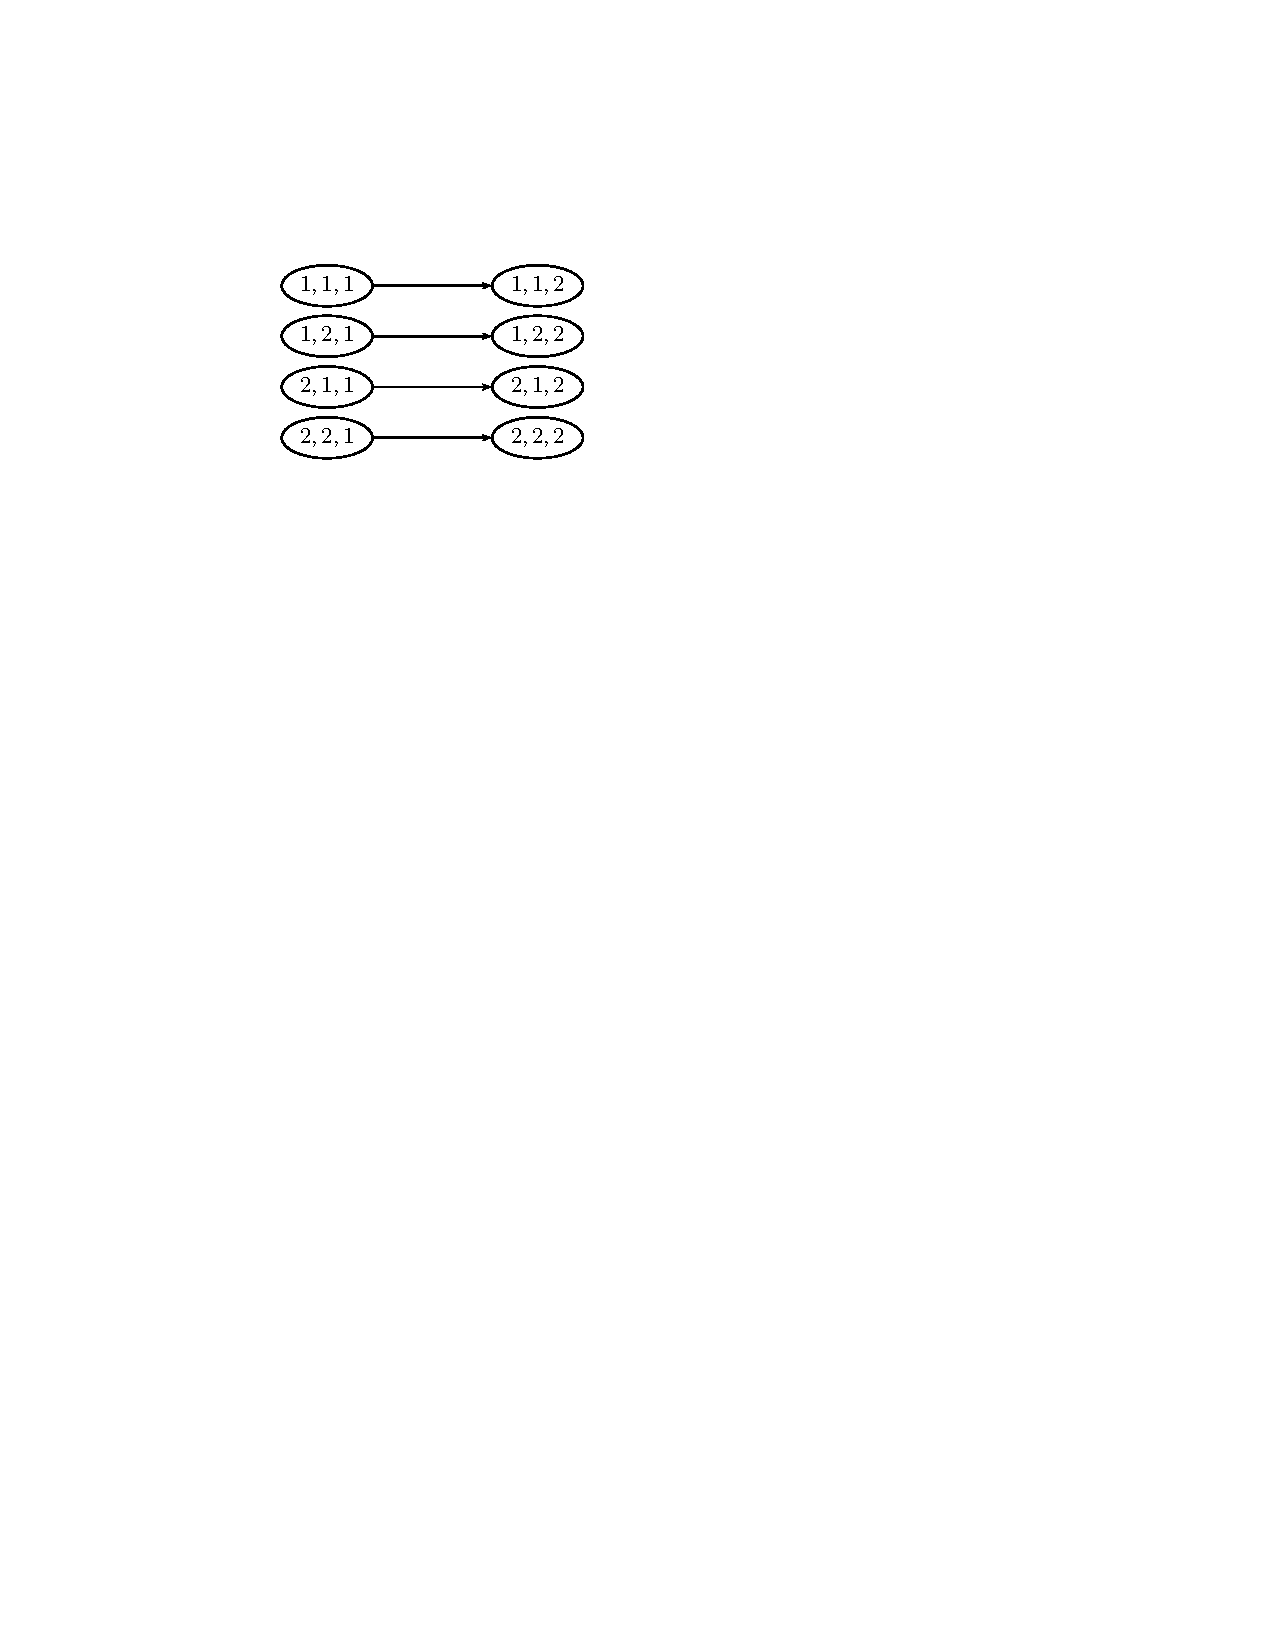
\includegraphics{figures/dag_gemm_22.pdf}
  \caption{Graphe de tâches induit pour un produit matriciel.}
  \label{fig:dag-gemm-22}
\end{figure}

Dans le cas où $n = 2$ dans l'algorithme précédent, le graphe de tâches est donné par la figure~\ref{fig:dag-gemm-22}, sur laquelle la tache $(i, j, k)$ représente l'opération (séquentielle) $C_{ij} \gets C_{ij} + A_{ik} B_{kj}$.
L'ordre d'exploration du graphe n'est pas spécifié, et 4 parties connexes donc totalement indépendantes du point de vue de l'exécution apparaissent.
\end{example}

\begin{rmq}[Accumulation]
  \label{rmq:reduction}
  Dans l'exemple précédent, les tâches dans la boucle la plus interne sont commutatives\footnote{En arithmétique exacte}.
  L'expression des dépendances formulée dans l'exemple précédent ne permet pas d'exposer cette caractéristique.
  Il est possible dans certains moteurs d'exécution (y compris QUARK et StarPU) de donner cette indication, sans laquelle les tâches de la boucle la plus interne ont des dépendances trop fortes (ordre strict au lieu d'exclusion mutuelle).
\end{rmq}

\subsection{Principes de base}
\label{sec:principes-de-base}
Le moteur d'exécution comprend quatres parties principales~:
\begin{enumerate}
\item Création du graphe de tâches à partir des appels à \texttt{insert\_task()}~;
\item Détermination des tâches éligibles à l'exécution~;
\item Ordonnancement des tâches éligibles~;
\item Gestion des \emph{workers}.
\end{enumerate}

\subsubsection{Construction du graphe de tâches}
\label{sec:constr-du-graphe}
La première étape (construction du graphe se décompose ici de la manière suivante)~:
\begin{itemize}
\item Construction des ensembles de dernier écrivain et derniers lecteurs à l'insertion des tâches~;
\item Ajout des arêtes et des sommets au graphe de tâche.
\end{itemize}

Une fois le graphe de tâche déterminé, les structures de données nécessaires aux étapes suivantes sont construites.
Plus précisément, les structures de données sont similaires à celles nécessaires pour effectuer un \textbf{tri topologique} d'un graphe acyclique dirigé.
Pour chaque sommet du graphe, on construit~:
\begin{itemize}
\item Le degré entrant de l'arête (pour le sommet $t_i$, nombre d'arêtes de la forme $t_j \to t_i$ dans le graphe)~;
\item La liste des successeurs de $t_i$, \emph{i.e.} l'ensemble $\{t_k \ |\ t_i \to t_k\}$.
\end{itemize}

\subsubsection{Détermination des tâches éligibles à l'exécution}
\label{sec:determ-des-tach}
Les tâches éligibles sont les sommets du graphe dont le degré entrant est égal à 0.
On note que ceci ne permet de construire que l'ensemble des tâches éligibles au début de l'exécution, il sera nécessaire de remettre à jour les structures de données au cours de l'exécution pour déterminer les autres tâches éligibles.
Par ailleurs, cet ensemble est non vide, puisque la première tâche insérée n'a pas de dépendance.

\subsubsection{Ordonnancement des tâches éligibles}
\label{sec:ordonn-des-tach}
Les tâches éligibles sont ajoutées à un ensemble de tâches dont l'exécution est possible, en attente de gestion par un des \emph{worker}.
L'ordre d'exécution effectif de ces tâches est laissé libre, puisqu'il ne peut pas avoir d'influence sur le résultat de l'algorithme, du fait de l'expression des dépendances supposée exhaustive dans le graphe de tâches.
Le modèle le plus simple est celui d'une simple file d'attente \ac{fifo}, mais d'autres politiques d'ordonnancement sont possibles.
Néanmoins, du point de vue du reste du moteur d'exécution, l'ordonnanceur fournit deux opérations~:~
\begin{itemize}
\item \texttt{push(task)}~:~ajoute une tâche à l'ensemble des tâches disponibles~;
\item \texttt{try\_pop()}~:~tente de récupérer une tâche, l'enlevant ainsi de l'ensemble des tâches en attente.
\end{itemize}
La première opération est appelée par le mécanisme de résolution des dépendances, la seconde par un des \emph{workers}.

\begin{figure}
  \centering
  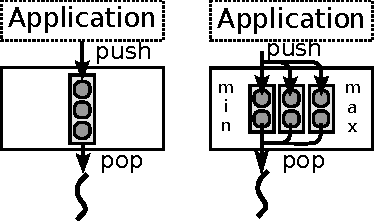
\includegraphics[width=8cm]{figures/eager-prio-starpu.pdf}
  \caption{Ordonnancement sans (\texttt{eager}) et avec priorités (\texttt{prio}).}
  \label{fig:eager-prio-starpu}
\end{figure}
Deux exemples d'ordonnanceurs sont illustrés par la figure~\ref{fig:eager-prio-starpu}, un ordonnanceur étant une simple \ac{fifo}, le second prenant en compte des priorités relatives entre les tâches.


\subsubsection{Gestion des workers}
\label{sec:gestion-des-workers}
Le c\oe{}ur du moteur d'exécution instancie un nombre configurable de \emph{workers}, typiquement un par c\oe{}ur sur la machine.
Chaque \emph{worker} est un \emph{thread}, créé et terminé dans \texttt{go()}, exécutant la boucle de l'algorithme~\ref{alg:boucle-worker}:

\begin{algorithm}[!htpb]
    \begin{algorithmic}
    \While{\textbf{true}}
    \State $ok \gets \texttt{try\_pop(t)}$
    \If{$\lnot ok$}
    \State \texttt{exponential\_backoff()}
    \State \textbf{continue}
    \EndIf
    \If{$t == \mathtt{SENTINEL}$}
    \State \textbf{break}
    \EndIf
    \State \Call{Execute}{$t$}
    \State \Call{UpdateDependencies}{$t$}
    \EndWhile
  \end{algorithmic}
  \caption{\label{alg:boucle-worker}Boucle d'exécution de tâches par un processeur.}
\end{algorithm}

Dans cet algorithme, la fonction \textsc{UpdateDependencies} est la fonction responsable de la mise à jour des structures de dépendances.
Plus précisément, elle retire la tâche $t$ du graphe de tâches, et ajoute les tâches nouvellement éligibles à la file d'attente.

\section{Runtime}
\label{sec:runtime}
Le moteur d'exécution est écrit en C++11, et n'a de dépendance que sur un compilateur C++11, la STL associée et MPI pour la mémoire distribuée.
Il repose essentiellement sur les classes suivantes~:~
\begin{itemize}
\item Classes ``externes''
  \begin{itemize}
  \item \texttt{TaskScheduler}~:~Singleton exposant les fonctions membre \texttt{insertTask()} et \texttt{go()}~;
  \item \texttt{Task}
  \end{itemize}
\item Classes ``internes''~:~
  \begin{itemize}
  \item \texttt{Scheduler}~:~politique d'ordonnancement, exposant \texttt{push()} et \texttt{tryPop()}
  \item \texttt{Worker}
  \end{itemize}
\end{itemize}

De plus, la gestion de MPI et de l'OOC a nécessité l'ajout d'une classe \texttt{Data} représentant une donnée, qui n'est pas présente dans les premières version, fonctionnant uniquement en mémoire partagée.

\subsection{Insertion des tâches}
\label{sec:insertion-des-taches}

\subsubsection{Tâches}
\label{sec:taches}
Les tâches sont dans \textsc{runtime} des classes dérivées de la classe \texttt{Task}, une classe abstraite de base, dont les éléments publics sont~:~
\begin{lstlisting}
class Task {
public:
  Priority priority;
  Task(std::string name="Task");
  virtual void call() = 0;
};
\end{lstlisting}
Autrement dit, une tâche est une classe ayant une méthode \texttt{call()} permettant d'exécuter la tâche.
Les paramètres de cette tâche doivent être passés autrement, par exemple dans le constructeur de la classe dérivée.

Une instance de \texttt{Task} est allouée par le code appelant, en revanche la destruction est assurée par le moteur d'exécution.

Par exemple, une tâche \texttt{GemmTask} peut être implémentée ainsi~:
\begin{lstlisting}
class GemmTask : public Task {
private:
  double alpha, beta;
  double *c, *a, *b;

public:
  GemmTask(double* c, double alpha, double* a, double* b, double beta)
    : alpha(alpha), beta(beta), c(c), a(a), b(b) {}
  void call() {
    cblas_dgemm(...);
  }
};
\end{lstlisting}

\subsubsection{InsertTask}
\label{sec:inserttask}

\paragraph{Utilisation}
\label{sec:utilisation}
Le prototype de la fonction membre \texttt{insertTask()} est~:~
\begin{lstlisting}
enum AcessMode {READ, WRITE};
void insertTask(Task* task, const vector<pair<Data*, AccessMode>>& params);
\end{lstlisting}
et peut être utilisée (en C++11) ainsi~:
\begin{lstlisting}
TaskScheduler s;
s.insertTask(new GemmTask(c, alpha, a, b, beta),
             {{a, READ}, {b, READ}, {c, WRITE}});
\end{lstlisting}
en supposant que le type \texttt{Data} est un alias de \texttt{void}.

\paragraph{Description}
\label{sec:description}
Le suivi des accès aux données est fait au travers de la class \texttt{AccessTracker} et du membre \texttt{dataAccess}~:
\begin{lstlisting}
struct AccessTracker {
  Task* lastWrite;
  deque<Task*> lastReads;
};
unordered_map<Data*, AccessTracker> dataAccess;
\end{lstlisting}
La classe \texttt{AccessTracker} suit le dernier accès en écriture et les derniers accès en écriture à une donnée, et \texttt{dataAccess} fait le lien entre une donnée et les accès.

Pour chaque dépendance \texttt{Data* d} d'une tâche \texttt{Task* t}, selon le type d'accès~:
\begin{description}
\item[READ] Si \texttt{dataAccess[d].lastWrite != NULL}, alors ajouter une dépendance \texttt{dataAccess[d].lastWrite} $\to$ \texttt{t}, et ajouter \texttt{t} à \texttt{dataAccess[d].lastReads}~;
\item[WRITE] Ajouter des dépendances~:
  \begin{itemize}
  \item \texttt{dataAccess[d].lastWrite} $\to$ \texttt{t}
  \item \texttt{t2} $\to$ \texttt{t} pour tout \texttt{t2} dans \texttt{dataAccess[d].lastReads}
  \end{itemize}
  Puis vider \texttt{dataAccess[d].lastReads}, et faire \texttt{dataAccess[d].lastwrite}~$\gets$~\texttt{t}
\end{description}

Toutes les dépendances de toutes les tâches sont collectées dans le membre \texttt{vector<pair<Data*, Data*>{}> deps} qui est l'ensemble des arêtes du graphe de tâches.

\subsection{Exécution}
\label{sec:execution}
Une fois toutes les tâches insérées, \texttt{TaskScheduler::go(nThreads)} est appelé.
Cette fonction doit~:
\begin{itemize}
\item Préparer les structures de données et les tâches initialement disponibles~;
\item Lancer les \emph{workers}
\item Attendre la fin de l'exécution.
\end{itemize}

\subsubsection{Préparation}
\label{sec:preparation}
L'étape précédente permet de construire le graphe de tâches.
Il est ensuite nécessaire de préparer les structures de données importantes pour le suivi des dépendances, ce qui est fait dans \texttt{TaskScheduler::prepare()}.
Les informations à suivre sont~:
\begin{itemize}
\item Degré entrant des sommets~;
\item Liste des successeurs.
\end{itemize}
Ces informations sont dans \texttt{map<Task*, TaskSuccessor> succ}, avec
\begin{lstlisting}
struct TaskSuccessors {
  int count; // degre entrant
  deque<Task*> successors;
};
\end{lstlisting}

La construction de cette structure est simple~:~
\begin{itemize}
\item Pour tout $t_i \to t_j \in \mathtt{deps}$,
  \begin{itemize}
  \item \texttt{succ[$t_j$].count += 1}
  \item \texttt{succ[$t_i$].successors.push\_back($t_j$)}
  \end{itemize}
\end{itemize}

Une fois cette structure construite, le graphe de tâche est inutile.
Toutes les tâches ayant pour degré entrant $0$ sont poussées dans la liste des tâches disponibles.

\subsubsection{Workers}
\label{sec:workers}
Un \texttt{worker} est une instance de cette classe~:
\begin{lstlisting}
class Worker {
private:
  Scheduler& q;
  TaskScheduler& scheduler;

public:
  Worker(Scheduler& q, TaskScheduler& scheduler);
  void mainLoop();
};
\end{lstlisting}
\texttt{Scheduler} est ici l'ordonnanceur (par exemple, \ac{fifo} ou avec gestion des priorités) qui est un conteneur intérieurement synchronisé (les fonctions membres \texttt{push} et \texttt{tryPop} sont plus ou moins équivalentes à des méthodes \texttt{synchronized} en Java).
La fonction membre \texttt{mainLoop()} implémente l'algorithme~\ref{alg:boucle-worker}, et la valeur sentinelle est \texttt{NULL}~;~c'est celle qui est lancée par le moteur d'exécution à la création du \textsc{thread}.

Les lignes importantes de cette fonction sont~:
\begin{lstlisting}
task->call();
scheduler.postTaskExecution(task);
\end{lstlisting}

La première est l'appel à la tâche, qui n'a besoin d'aucune synchronisation.
La seconde est la mise à jour des dépendances et la libération de \texttt{t}.

\subsubsection{Mise à jour des dépendances}
\label{sec:mise-jour-des}
Lorsqu'une tâche à été exécutée, elle est retirée du graphe de tâches.
Ceci correspond à décrémenter le degré entrant de tous ses successeurs, ce qui est fait dans \texttt{TaskScheduler::postTaskExecution()}.
Puisque cette fonction peut être appelée par n'importe quel \emph{worker}, elle est protégée par un \emph{mutex}.

Plus précisément~:
\begin{itemize}
\item Pour toutes les tâches $t_2$ dans \texttt{succ[$t$].successors}
  \begin{itemize}
  \item \texttt{succ[$t_2$].count-{}-}~;
  \item Si \texttt{succ[$t_2$].count == 0}, on l'ajoute dans la liste des tâches prêtes.
  \end{itemize}
\end{itemize}

Le reste de la fonction s'occupe de nettoyage des structures, et de vérifier qu'il reste encore des tâches à exécuter.
Dans le cas contraire, une tâche ``sentinelle'' (\texttt{NULL} ici) est poussée par \emph{worker}, de manière à signaler la terminaison.
C'est également cette fonction qui détruit l'instance de la tâche.

\subsubsection{Verrouillage}
\label{sec:verrouillage}
Il y a peu de verrous dans le moteur d'exécution.
En effet, l'exécution des tâches ne nécessite aucun verrouillage, sous réserve que les dépendances de données soient correctement spécifiées.
Les élements nécessitant une protection sont~:~
\begin{itemize}
\item L'ordonnanceur. L'opération \texttt{push()} n'est appelée que par un \emph{thread} à la fois puisque son accès est fait depuis \texttt{postTaskExecution()}.
  En revanche, l'opération \texttt{tryPop()} est appelée par tous les \emph{workers}, et doit être protégée.
\item Les structures contenant les dépendances entre les tâches, modifiées par \texttt{postTaskExecution()}.
\end{itemize}

\paragraph{Ordonnanceur}
\label{sec:ordonnanceur}
Extérieurement, l'ordonnanceur est une file d'attente de type \emph{Single Producer, Multiple Consumers} (SPMC).
Elle est néanmoins implémentée ici comme une file d'attente synchronisée intérieurement, et supportant un modèle \emph{Multiple Producers, Multiple Consumers} (MPMC).
De plus, il n'y a qu'un seul verrou pour les écrivains et les lecteurs, ce qui n'est pas optimal, mais plus simple.

\paragraph{Gestion des dépendances}
\label{sec:gest-des-depend}
Tous les appels à \texttt{postTaskExecution()} sont protégés par un \emph{mutex}, ce qui donne l'équivalent d'une méthode \texttt{synchronized} en Java.




\end{document}


%%% Local Variables: 
%%% mode: latex
%%% TeX-master: t
%%% End: 
